\chapter{Cloud Computing}
\label{ch:cloud_computing}

Cloud Computing is both applications available over the internet, but also the hardware and system software that provide these services.
Rather than scaling a single node vertically, Cloud Computing shifts focus and enables horizontal scaling of virtualized storage and network resources\cite{armbrust2010view}. Cloud computing enable applications to fulfil new requirements for rapid capacity up and down scaling, with the notion that available virtual resources are limitless\cite{sosinsky2010cloud}.

According to \citeauthor{sosinsky2010cloud} Cloud Computing sets new standards for system development and deployment, representing a real paradigm shift:\\
\begin{quote_highlight}
"Cloud computing represents a real paradigm shift in the way in which systems are deployed. The massive scale of cloud computing systems was enabled by the popularization of the Internet and the growth of some large service companies. Cloud computing makes the long-held dream of utility computing possible with a pay-as-you-go, infinitely scalable, universally available system. [...] That’s why cloud computing is revolutionary, even if the technology it is built on is evolutionary"\cite[p. 3 ]{sosinsky2010cloud}
\end{quote_highlight}\\

Cloud Computing is a enabler for further evolving how distributed systems are designed, distributed, updated and accessed.

\section{Defining Cloud Computing}
This section will try and pin down what defines Cloud computing, enabling usage of the term for the rest of the report. Cloud Computing has been over utilized, and the term has become very saturated.

The National Institute of Standards and Technology (NIST) defines Cloud Computing\\
\begin{definition}
Cloud computing is a model for enabling ubiquitous, convenient, on-demand network access to a shared pool of configurable computing resources\citeauthor{mell2011nist}
\end{definition}
\\
Cloud infrastructures are a composition of hardware and software enabling five essential characteristics. Each characteristic is detailed below.

\textbf{On-demand self-service}\\
Computing capabilities can be provisioned on-demand automatically without human interaction.


\textbf{Broad network access}\\
Capabilities are heterogeneous accessible over the network.


\textbf{Resource pooling}\\
The providers computing resources are pooled, serving multiple consumers simultaneously. Different physical and virtual resources are dynamically assigning and reassigning based on consumer demand.


\textbf{Rapid elasticity}\\
Capabilities are elastic, supporting rapid outward and inward scaling. 


\textbf{Measured service}\\
Resources are measured, providing transparency for both the provider and consumer. Enabling cloud systems to optimize resource usage.


\comment{Maybe include this in the definition?}


Three aspects introduced with Cloud Computing: \cite{armbrust2010view}
1. Infinite computing resources available on demand. Can help dealing with load surges, nullifying the need for provisioning planning.
2. Only increasing hardware resources when needed.
3. paying for computing resources as you go.

Three defining aspects\cite{sosinsky2010cloud}.
1. Abstraction
2. Massively scalable
3. Utility, service provided

\begin{figure}[!htb]
  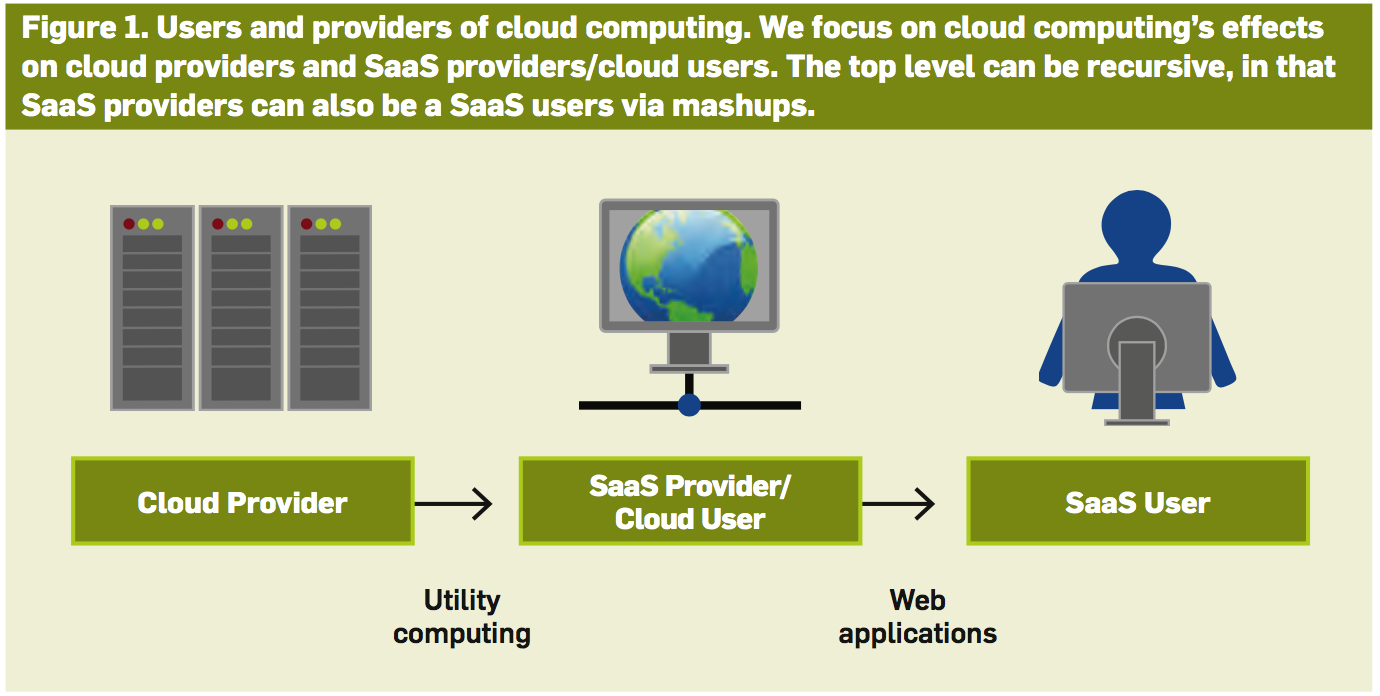
\includegraphics[scale=0.5]{cloud_computing_definition_cloud_infrastructure}  
  \caption{Cloud infrastructure}
  \label{fig:cloud_computing_definition_cloud_infrastructure}
\end{figure}

\subsection{Service models / Utility Computing Classes}
The aforementioned cloud infrastructure characteristics is made available to the consumer through three different service models\cite{mell2011nist}.
Service models are distinguished by the provided systems software abstraction and resource management level. The level of abstraction and resource management affect the available services, leaving increasing levels of management responsibilities to the provider\cite[p. 52]{armbrust2010view}.
The three service models are depicted on figure \ref{fig:cloud_computing_definition_service_models}, where the different abstraction levels are visible.

\textbf{Software as a Service (SaaS)}\\
Provider make complete applications availbe on the cloud infrastructure, for consumers to start up. The applications are accessible through thin client interfaces (eg. web browsers), or program interfaces. The consumer does not manage or control underlying infrastructure and is therefore alleviated the burden of maintenance, operation and support costs \cite{youseff2008toward}.


\textbf{Platform as a Service (PaaS)}\\
The consumer can deploy consumer-created or acquired applications, controlling the deployment and potentially configuration settings for the hosting environment. Underlying cloud infrastructure network, servers storage, virtualization, operating system and runtime is provider managed.

\textbf{Infrastructure as a Service (IaaS)}\\
The consumer can provision processing, storage and network resources, but does not manage them. The consumer can run arbitrary software.

\begin{figure}[!htb]
  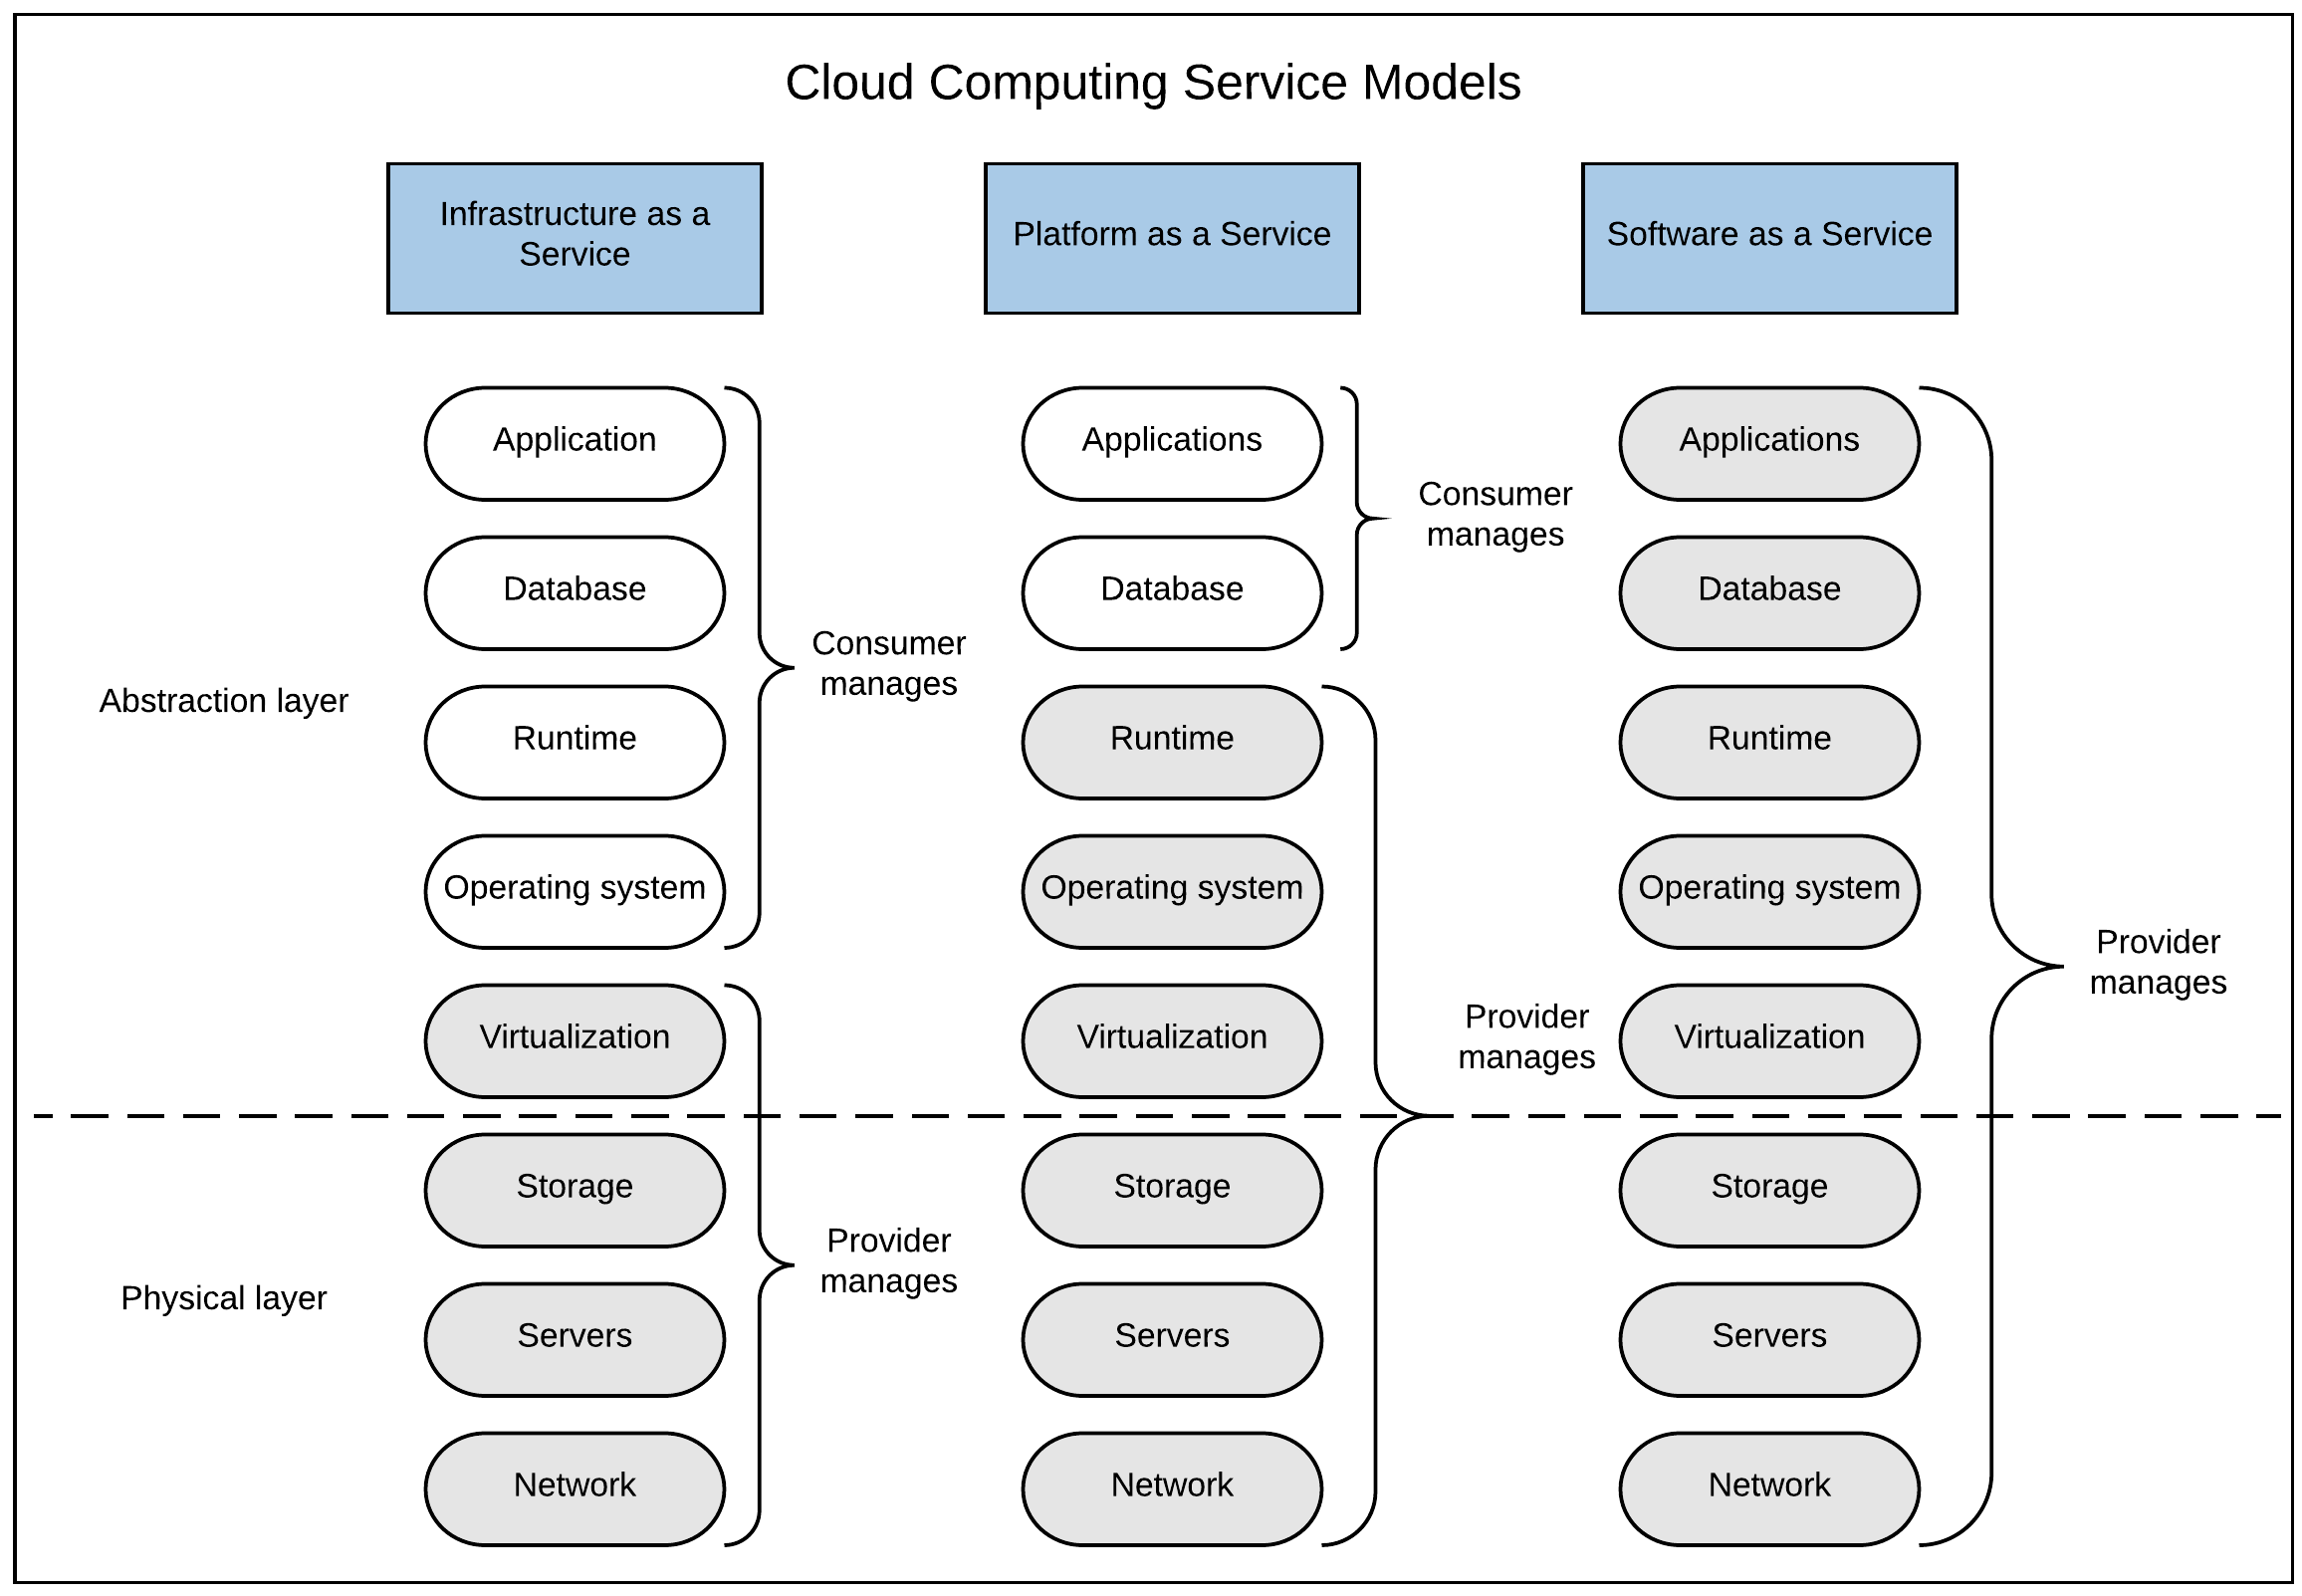
\includegraphics[scale=0.15]{cloud_computing_definition_service_models}  
  \caption{Service models}
  \label{fig:cloud_computing_definition_service_models}
\end{figure}

\comment{Notes}
utility computing - the computer resources being sold

Virtualization makes management and automatic allocation of resources possible, giving the possibility to create very adaptable applications where capacity can be infinitely increased on demand\cite{armbrust2010view}.

Utility computing, 

Any application needs a model computation, storage and communication. 


"Service models describe the type of service that the service provider is offering. The best-known service models are Software as a Service, Platform as a Service, and Infrastructure as a Service—the SPI model. The service models build on one another and define what a vendor must manage and what the client’s responsibility is."


\subsection{Deployment models}
Cloud infrastructures are made available through four different deployment models, with distinct differences. The deployment model describes  location and ownership of the infrastructure, and determines who is responsible for the infrastructure. The deployment model affects the expected data confidentiality and security, the specified availability, and the available deployment size.


\textbf{Private cloud}\\
Internal data center, provisioned for exclusive use to the owning organization.


\textbf{Community cloud}\\
The infrastructure is provisioned exclusively to a community of organizations with shared concerns to mission, security and policy among others.


\textbf{Public cloud}\\
The cloud infrastructure is provisioned to the general public, in a "Pay-as-you-go" manner.

\textbf{Hybrid cloud}\\
A composition of several distinct cloud infrastructures.


\citeauthor{armbrust2010view} states that data confidentiality and auditability is one of the biggest obstacles, for a large-scale adoption of public cloud computing infrastructures. Internal consumer concerns and legislation prohibits some consumers from fully adopting public cloud computing infrastructures, forcing a private cloud deployment models. 
\comment{Should this be here or somewhere else? Should it be expanded?}


\section{Virtualization}
"Cloud computing bible"
"Given a computer system with a certain set of resources, you can set aside portions of those resources to create a virtual machine. From the standpoint of applications or users, a virtual machine has all the attributes and characteristics of a physical system but is strictly software that emulates a physical machine."\cite[p. 100]{sosinsky2010cloud}



\section{Cluster management}

\url{https://www.nomadproject.io/intro/vs/ecs.html}

\subparagraph{Kubernetes}

\url{https://kubernetes.io/docs/whatisk8s/}

\section{Containerization}


\subsection{Docker}

\subsection{RKT}
\url{https://aptira.com/coreos-rkt/}

\subsection*{Noter}
\url{https://en.wikipedia.org/wiki/Cloud_computing#Infrastructure_as_a_service_.28IaaS.29}

Infrastructure as a service  (IaaS)

Platform as a service (Paas) \url{https://en.wikipedia.org/wiki/Platform_as_a_service}

Software as a service (SaaS)

Mobile backend as a service MBaaS \url{https://en.wikipedia.org/wiki/Mobile_backend_as_a_service}

DevOps

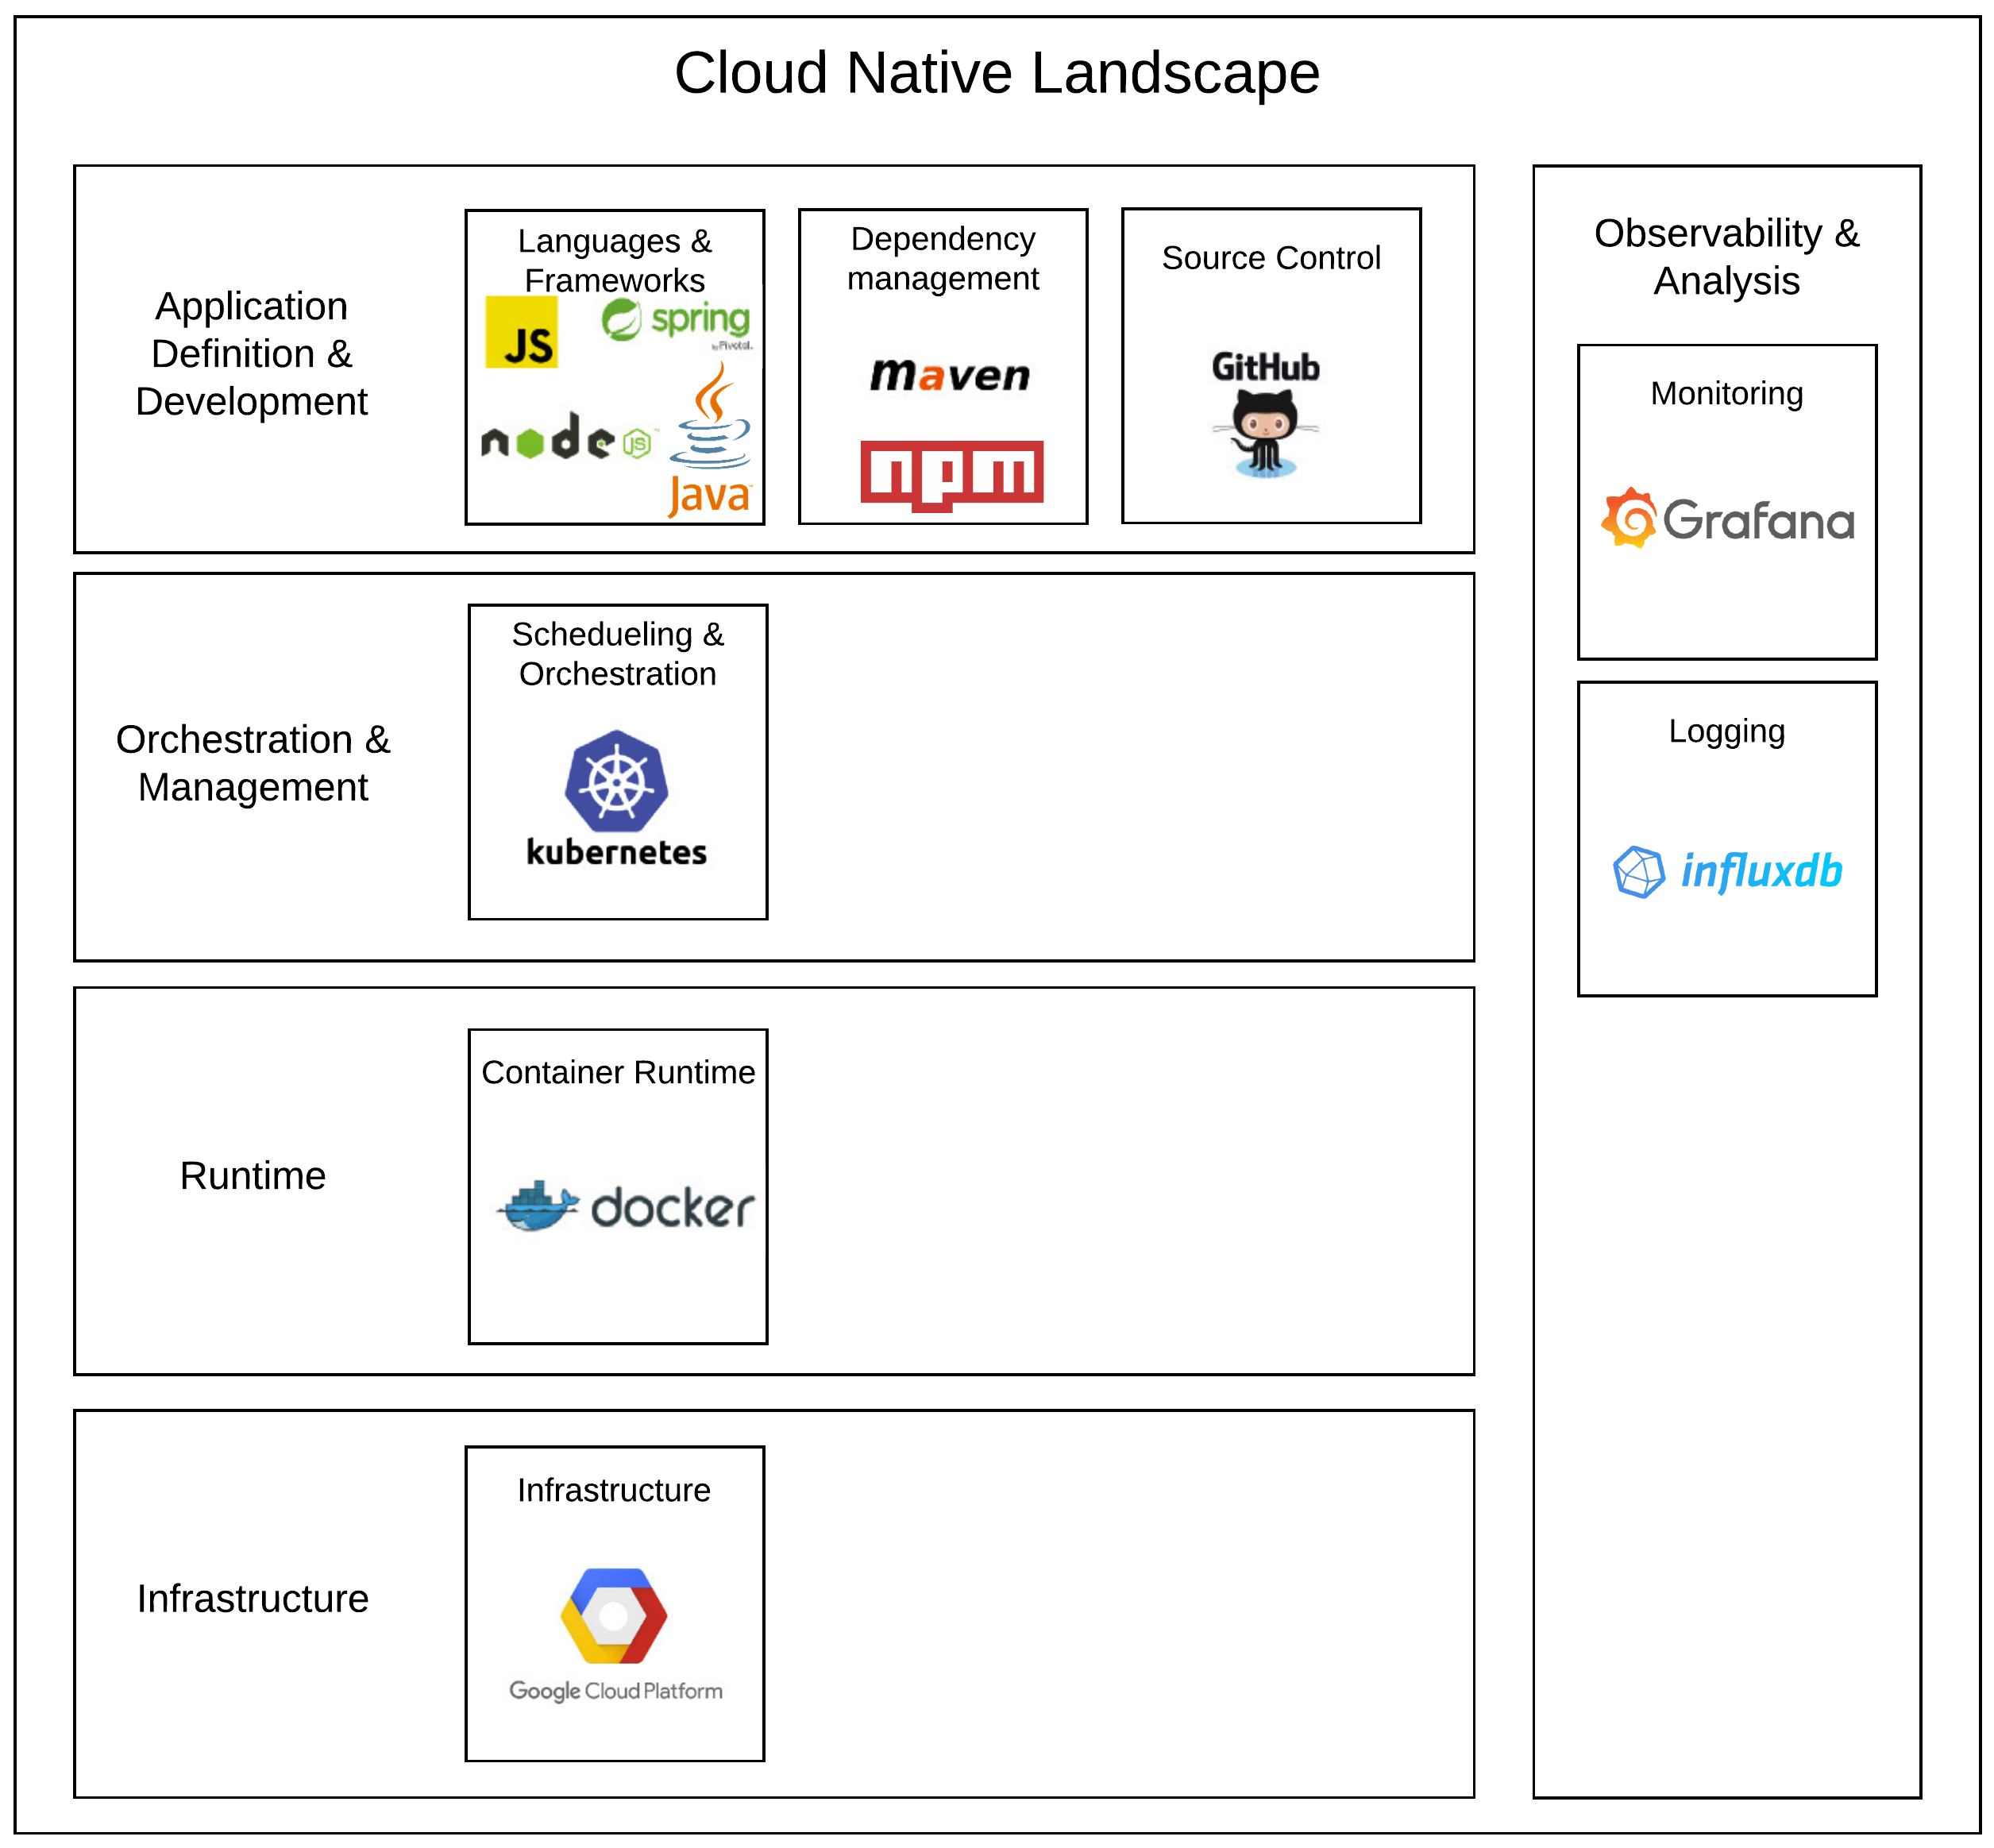
\includegraphics[scale=0.12]{cloud_computing_cloud_native_landscape}

\subsection*{Notes}
Service Oriented Architectures \url{https://en.wikipedia.org/wiki/Service-oriented_architecture}